\section{Aplicación del Código de Medida} \label{sec:aplicacion}
La empresa \textbf{ENERGER S.A} llevará a cabo la puesta en marcha de una \textbf{planta generadora hidráulica de 975 MW}, que se compone de un grupo generador e instalaciones de operación (incluyendo servicios auxiliares).

El \textbf{grupo generador} estará conformado por tres generadores síncronos monofásicos de \textbf{325 MVA, 15 kV, 60 Hz y 8 polos}, el cual inyectará la potencia generada al \textbf{STN} a través de un transformador de \textbf{1000 MVA, 15 kV / 230 kV} y conexión \textbf{Dd6}. Las \textbf{instalaciones de operación} de la planta generadora operarán a \textbf{13.8 kV} y serán alimentadas directamente desde el STN a través de un transformador de \textbf{500 kVA, 230 kV / 13.8 kV} y conexión \textbf{Dd6}.

Se debe tener en cuenta la siguiente información. La planta generadora opera según \textbf{tres regímenes o intervalos}, tanto en el grupo generador como en las instalaciones de operación.

\begin{table*}[t]
  \centering
  \caption{Regímenes de operación de la planta generadora.}
  \label{tab:regimenes_operacion}
  \begin{tabular}{ccccccc}
    \toprule
    \multirow{2}{*}{\textbf{Intervalo}} & \multicolumn{3}{c}{\textbf{Grupo generador}} & \multicolumn{3}{c}{\textbf{Instalaciones de operación}} \\
    \cmidrule(lr){2-4} \cmidrule(lr){5-7}
    & \textbf{Tiempo} & \textbf{Generación} & \textbf{fp} & \textbf{Tiempo} & \textbf{Consumo} & \textbf{fp} \\
    \midrule
    1 & 50\% & 85\% & 1.0 & 45\% & 85\% & 0.92 ad \\
    2 & 45\% & 80\% & 0.95 at & 50\% & 90\% & 0.95 ad \\
    3 & 5\% & 50\% & 0.91 at & 5\% & 70\% & 0.95 ad \\
    \bottomrule
  \end{tabular}
\end{table*}

Debido a la disposición física de la planta generadora, la distancia entre los transformadores de medida correspondientes al grupo generador y el gabinete del sistema de medición es aproximadamente $l_1= \mathbf{225 \text{ m}}$; mientras esta distancia es aproximadamente $l_2 = \mathbf{120 \text{ m}}$ entre los transformadores de medida correspondientes a las instalaciones de operación y el gabinete del sistema de medición.

Con base en un análisis técnico-financiero, se definió que el esquema de medición deberá brindar la siguiente información: \textbf{(i) energía generada (activa y no activa)} por parte del grupo generador y \textbf{(ii) energía consumida (activa y no activa)} debida a las instalaciones para la operación del grupo generador.

El reporte de diseño del sistema de medición deberá contener como mínimo la siguiente información: \textbf{Definición de los tipos de frontera}, \textbf{Definición de los tipos de punto de medida}, \textbf{Cantidad, tipo y clase de medidores y transformadores de medida requeridos} de acuerdo con los tipos de frontera seleccionados, \textbf{Esquema de conexión de los sistemas de medición}, \textbf{Selección de los transformadores de medición. Análisis de alternativas}, \textbf{Análisis de la incertidumbre máxima} que se presentará en la medición de las energías activa y de la potencia (energía) reactiva de acuerdo con el tipo de frontera comercial analizado, y \textbf{Análisis de las especificaciones del sistema de medición y su cumplimiento} con las exigencias del código de medida con relación al \textbf{Burden} de los transformadores de medida y la \textbf{caída de tensión} que se presenta en los conductores del secundario de los transformadores de medida.

\subsection{Tipos de Frontera} \label{subsec:tipos_frontera}
\begin{itemize}
    \item \textbf{Fronteras de generación}: Corresponde al punto de medición de una unidad o planta de generación donde las transferencias de energía equivalen a la energía neta entregada por el generador al STN, al STR o al SDL.
    \item \textbf{Fronteras de comercialización}: Punto de medición donde las transferencias de energía registradas permiten determinar la demanda de energía de un comercializador. A su vez, se clasifican en:
    \begin{itemize}
        \item \textbf{Frontera de comercialización entre agentes}: Permite determinar la transferencia de energía entre mercados de comercialización o entre el STN y un mercado de comercialización.
        \item \textbf{Frontera de comercialización entre agentes y usuarios}: Corresponde a toda frontera de comercialización que no cumple con los criterios de la frontera entre agentes. También incluye la frontera comercial de un usuario que se conecta directamente al STN.
    \end{itemize}
\end{itemize}

\subsection{Definición de los Tipos de Punto de Medida} \label{subsec:tipos_punto_medida}
Partiendo de la capacidad instalada por los generadores, y según la \textbf{Tabla 1 del artículo 6 de la resolución CREG 038} se puede determinar que el tipo de punto de medición tanto para generaciones como para instalación de operación es \textbf{Tipo 1}.

\begin{table*}[t]
  \centering
  \caption{Clasificación de puntos de medición.}
  \label{tab:clasificacion_puntos_medicion}
  \begin{tabular}{ccc}
    \toprule
    \textbf{Tipo de puntos de medición} & \textbf{Consumo o transferencia de energía, C [MWh-mes]} & \textbf{Capacidad Instalada, CI [MVA]} \\
    \midrule
    1 & $\ge 15.000$ \cellcolor{lightgreen} & $\ge 30$ \cellcolor{lightgreen} \\
    2 & $15.000 > C \ge 500$ & $30 > CI \ge 1$ \\
    3 & $500 > C \ge 50$ \cellcolor{lightred} & $1 > CI \ge 0,1$ \cellcolor{lightred} \\
    4 & $50 > C \ge 5$ & $0,1 > CI \ge 0,01$ \\
    5 & $C < 5$ & $CI < 0,01$ \\
    \bottomrule
  \end{tabular}
  \caption*{\textbf{Figura 1.} Tipos de puntos de medición.}
\end{table*}

En la tabla anterior está seleccionado con color \textbf{verde} el tipo de punto de medición para la \textbf{frontera de generación} y en color \textbf{rojo} el tipo de punto de medición para la \textbf{frontera de comercialización}. En este caso, como la frontera de generación nos da un tipo más alto, este es el que se elige para ambas fronteras.

\subsection{Cantidad, Tipo y Clase de Medidores y Transformadores de Medida Requeridos} \label{subsec:cantidad_clase_medidores}
Según lo establecido en la resolución CREG 038 de 2014, los tipos de frontera de generación y comercialización deben contar con un \textbf{medidor principal y uno de respaldo}. Además, el medidor de respaldo debe operar permanentemente y tener las \textbf{mismas características técnicas} que el medidor principal.

A continuación, se presenta la tabla para determinar la clase del medidor según su tipo de punto de medición:

\begin{table*}[t]
  \centering
  \small % Reducimos la fuente para ayudar a que quepa en doble columna
  \caption{Requisitos de exactitud para medidores y transformadores de medida.}
  \label{tab:requisitos_exactitud}
  \begin{tabular}{ccccc}
    \toprule
    \textbf{T. punto de medicion} & \textbf{Índ. de clase activa} & \textbf{Índ de clase reactiva} & \textbf{Exactitud para CTs} & \textbf{Clase de exactitud para TPs} \\
    \midrule
    1 & 0,2 S & 2 & 0,2 S & 0,2 \\
    2 y 3 & 0,5 S & 2 & 0,5 S & 0,5 \\
    4 & 1 & 2 & 0,5 & 0,5 \\
    5 & 1 ó 2 & 2 ó 3 & -- & -- \\
    \bottomrule
  \end{tabular}
  \caption*{\textbf{Figura 2.} Tabla de requisitos de exactitud para medidores y transformadores de medida.}
\end{table*}

\subsubsection{Medidores para la Frontera de Generación}
En la siguiente tabla se presentan los medidores de potencia activa y reactiva según su clase. Es importante resaltar que estos medidores deben ser idénticos para que puedan entrar en funcionamiento.

\begin{table*}[t]
  \centering
  \caption{Elección de la clase de medidor para la frontera de generación.}
  \label{tab:clase_medidor_generacion}
  \begin{tabular}{cccc}
    \toprule
    \textbf{MEDIDOR} & \textbf{CLASE} & \textbf{TRANSFORMADOR DE MEDIDA} & \textbf{CLASE} \\
    \midrule
    Activa & 0.2S & PT & 0.2 \\
    Reactiva & 2 & CT & 0.2S \\
    \bottomrule
  \end{tabular}
\end{table*}

\subsubsection{Medidores para la Frontera de Comercialización Entre Agente y Usuario}
En la siguiente tabla se presentan los medidores de potencia activa y reactiva según su clase. Es importante resaltar que estos medidores deben ser idénticos para que puedan entrar en funcionamiento.

\begin{table*}[t]
  \centering
  \caption{Elección de la clase de medidor para la frontera de comercialización.}
  \label{tab:clase_medidor_comercializacion}
  \begin{tabular}{cccc}
    \toprule
    \textbf{MEDIDOR} & \textbf{CLASE} & \textbf{TRANSFORMADOR DE MEDIDA} & \textbf{CLASE} \\
    \midrule
    Activa & 0.5S & PT & 0.5 \\
    Reactiva & 2 & CT & 0.5S \\
    \bottomrule
  \end{tabular}
\end{table*}

\subsection{Esquema de Conexión de los Sistemas de Medición} \label{subsec:esquema_conexion}
En sistemas eléctricos de $\mathbf{230 \text{ kV}}$, la medición siempre se realiza de forma \textbf{indirecta}, utilizando transformadores de corriente (TC) y de tensión (TT), conforme a lo establecido en la Resolución CREG 038 de 2014.

Cuando la carga está balanceada, la conexión del medidor se clasifica como \textbf{indirecta simétrica}, ya que las magnitudes de corriente y tensión en cada fase se mantienen proporcionales y dentro de los límites de exactitud exigidos por la normativa.

\begin{figure*}[t]
    \centering
    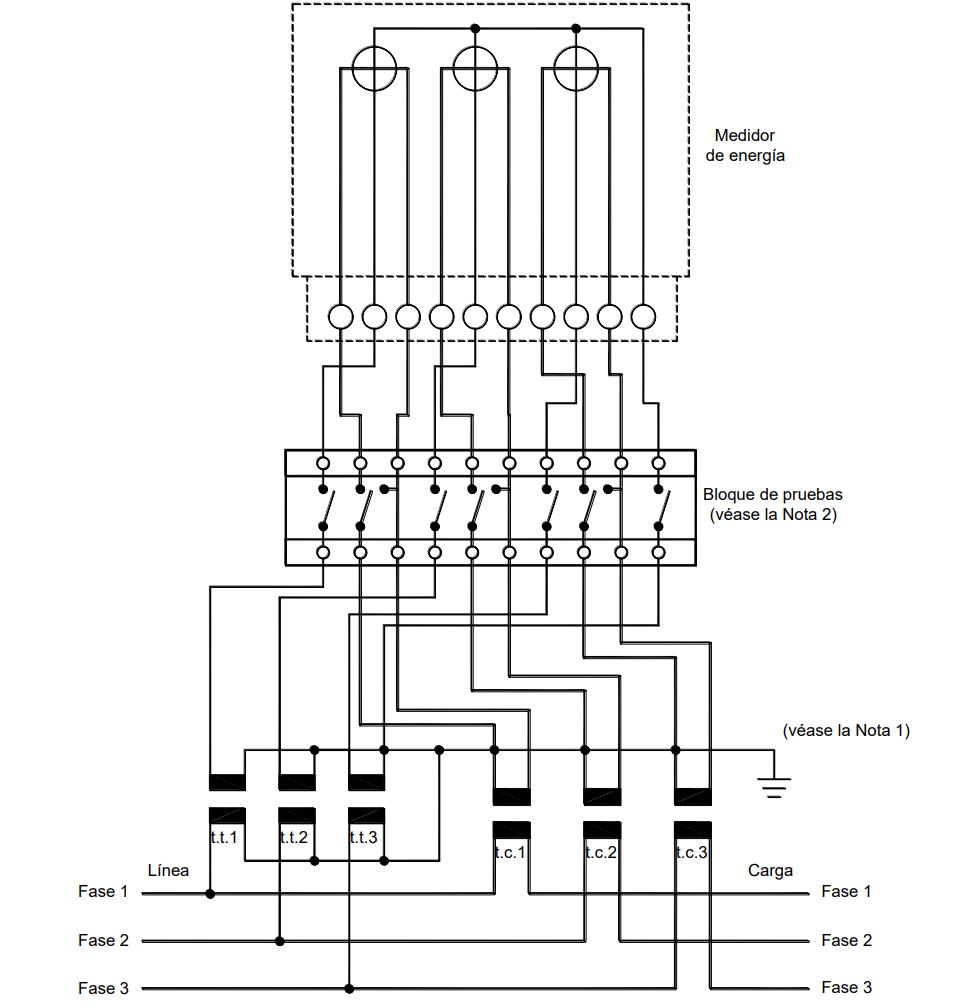
\includegraphics[width=\columnwidth]{figs/figura_esquema_simetrico.png}
    \caption{Esquema de conexiones medidor trifásico tetrafilar para medición indirecta entre tres elementos, conexión simétrica.}
    \label{fig:esquema_simetrico}
    \caption*{\textbf{Figura 3.} Esquema de conexión medición indirecta simétrica.}
\end{figure*}

Por el contrario, si la carga se encuentra \textbf{desbalanceada}, la conexión se considera \textbf{indirecta asimétrica}, debido a que las fases no presentan igualdad en magnitud ni en ángulo, generando registros de consumo diferentes entre ellas. Esta situación es contemplada por la CREG como una condición que exige selección y verificación adecuada de los transformadores de medida para garantizar la confiabilidad de la medición.

\begin{figure*}[t]
    \centering
    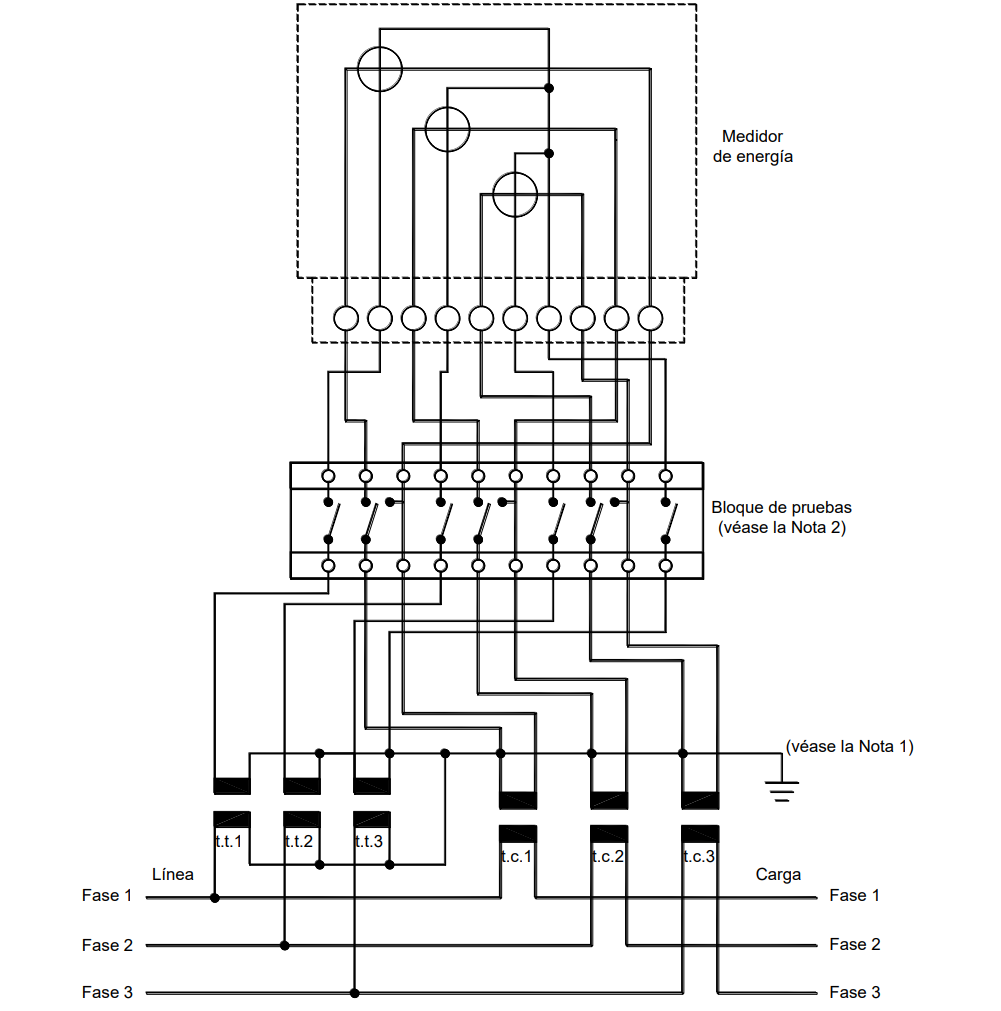
\includegraphics[width=\columnwidth]{figs/figura_esquema_asimetrico.png}
    \caption{Esquema de conexiones medidor trifásico tetrafilar para medición indirecta en tres elementos, conexión asimétrica.}
    \label{fig:esquema_asimetrico}
    \caption*{\textbf{Figura 4.} Esquema de conexión medición indirecta asimétrica.}
\end{figure*}

\subsection{Selección de los Transformadores de Medición. Análisis de Alternativas} \label{subsec:seleccion_transformadores}
\subsubsection{Frontera de Generación}
\begin{itemize}
    \item $S_{\text{generador}} = \mathbf{975 \text{ [MVA]}}$
    \item $V_{\text{nom}} = \mathbf{230 \text{ [kV]}}$
\end{itemize}

Calculamos la corriente nominal. La fórmula se muestra a continuación:
$$I_{\text{nom}} = \frac{S_{\text{generador}}}{\sqrt{3} \cdot V_{\text{nom}}} \text{ [A]} \text{}$$
Sustituyendo los valores:
$$I_{\text{nom}} = \frac{975 \text{ [MVA]}}{\sqrt{3} \cdot 230 \text{ [kV]}} \text{ [A]} \text{}$$
$$I_{\text{nom}} = \mathbf{2447,46 \text{ [A]}} \text{}$$
Con esto, calculamos el $I_{p'}$:
$$I_{p'} = C_T \cdot I_{\text{nom}} \quad; \quad C_T = 120\% \text{}$$
$$I_{p'} = 120\% \cdot 2447,46 \text{ [A]} \text{}$$
Con esta operación obtenemos un valor de $I_{p'}$ igual a:
$$I_{p'} = \mathbf{2936,952 \text{ [A]}} \text{}$$
Luego, buscamos los valores más cercanos de corriente que soporte los CT y aproximamos nuestro valor hallado al valor comercial:
$$R T_{CT} = \mathbf{3000:5} \text{}$$

\subsection{Análisis de la Incertidumbre Máxima en la Medición} \label{subsec:analisis_incertidumbre}
Se considera el siguiente aporte porcentual de error de los componentes:
\begin{itemize}
    \item Medidor de energía Activa 0.2S: $\mathbf{0.20 \ \%}$
    \item Medidor de energía Reactiva clase 2: $\mathbf{2.0 \ \%}$
    \item Transformador de Corriente CT clase 0.2S: $\mathbf{0.20 \ \%}$
    \item Transformador de Tensión clase 0.2: $\mathbf{0.20 \ \%}$
    \item Burden del CT: $\mathbf{0.16 \ \%}$
    \item E\% por cableado y conexiones: $\mathbf{0.10 \ \%}$
    \item E\% Fase Energía Reactiva: $\mathbf{0.03 \ \%}$
\end{itemize}

El \textbf{Burden en VA} se calcula como $V A_{\text{Burden}} = I_{\text{sec}}^2 \times R_{\text{line}}$.
\begin{itemize}
    \item Para el tramo de $\mathbf{225 \text{ m}}$ con $\mathbf{50 \text{ mm}^2}$: Con $I_{\text{sec}}=4.895 \text{ A}$ y $R_{\text{line}}=0.1552 \ \Omega$ se obtuvo un burden $\approx \mathbf{3.72 \text{ VA}}$.
    \item Para el tramo de $\mathbf{120 \text{ m}}$ con $\mathbf{25 \text{ mm}^2}$: Con $V=0.81013 \text{ V}$ y $R_{\text{line}}=0.1655 \ \Omega$ se obtuvo un burden $\approx \mathbf{3.97 \text{ VA}}$.
\end{itemize}
Dado que el CT está diseñado para $\mathbf{5 \text{ VA}}$, para el caso de $3.97 \text{ VA}$:
$$\frac{3.97}{5} = 0.794 \text{}$$
El error aumenta proporcionalmente: $0.2\% \times 0.794 = \mathbf{0.1588 \ \%}$.

\paragraph{Incertidumbre Total (Peor Caso y RMS)}
\begin{itemize}
    \item Suma directa de los $\%$ (Peor de los casos, Activa): $\mathbf{0.86 \ \%}$
    \item Suma de los RMS $\%$ (Para Activa): $\mathbf{0.39 \ \%}$
    \item Suma directa de los $\%$ (Reactiva - se agrega el de fase y el medidor de reactiva): $\mathbf{2.69 \ \%}$
    \item Suma de los RMS $\%$ (Para Reactiva): $\mathbf{2.03 \ \%}$
\end{itemize}

Para la frontera de \textbf{tipo 1}, compuesta por medidor principal y de respaldo clase $\mathbf{0.2S}$ (energía activa), clase $\mathbf{2}$ (energía reactiva), CT $\mathbf{3000:5}$ clase $\mathbf{0.2S}$ y PT clase $\mathbf{0.2}$, se evaluó la incertidumbre total considerando los errores de cada elemento y el efecto del \textbf{burden} en los conductores secundarios.

Los cálculos se realizaron con longitudes de $\mathbf{225 \text{ m} (50 \text{ mm}^2)}$ y $\mathbf{120 \text{ m} (25-35 \text{ mm}^2)}$, obteniendo un burden aproximado de $\mathbf{3.72 \text{ VA}}$, valor inferior al nominal de los transformadores, por lo que no genera sobrecarga ni incrementa el error del sistema. Combinando los errores de medidor, CT, PT y burden se obtiene:
\begin{itemize}
    \item Energía activa: incertidumbre total $\approx \mathbf{0.39 \ \%}$
    \item Energía reactiva: incertidumbre total $\approx \mathbf{2.03 \ \%}$
\end{itemize}
Estos valores \textbf{cumplen con los límites} establecidos por la Resolución CREG 038 de 2014 para fronteras tipo 1.

\subsection{Análisis del Burden y Caída de Tensión} \label{subsec:analisis_burden_caida_tension}
El sistema de medición \textbf{cumple} con lo que pide la Resolución CREG 038 de 2014, ya que el \textbf{burden total} de los transformadores de medida se mantiene dentro de los valores permitidos.

Para las distancias de $\mathbf{225 \text{ m}}$ y $\mathbf{120 \text{ m}}$, con conductores de $\mathbf{50 \text{ mm}^2}$ y $\mathbf{25-35 \text{ mm}^2}$, la \textbf{caída de tensión} en el secundario del CT es de más o menos $\mathbf{0.7 \text{ a } 0.8 \text{ V}}$, lo que equivale a un \textbf{burden} cercano a $\mathbf{3.7 \text{ VA}}$. Ese valor está \textbf{por debajo del nominal ($\mathbf{5 \text{ VA}}$)}, así que los transformadores trabajan en su rango correcto y conservan la clase de exactitud ($\mathbf{0.2S \text{ y } 0.2}$).

En conclusión, el sistema de medición \textbf{cumple} con el Código de Medida tanto en el \textbf{burden} como en la \textbf{caída de tensión} de los secundarios.